\chapter{Резюме на глава 2: Онтологията на OpenBiodiv}
\label{chapter-ontology}

OpenBiodiv трансформира информация за биоразнообразието от научни публикации и академични бази данни в семантичен вид. В тази глава представяме OpenBiodiv-O (\cite{senderov_openbiodiv-o:_2018}) -- онтологията, формираща модела на OpenBiodiv за знания и извод. OpenBiodiv-O предоставя концептуален модел на структурата на академична публикация в сферата на биоразнообразието и на съдържаните в нея таксономични концепции. За първи път формално е концептуализирана областта на публикуването на знание за биоразнообразието.

Чрез разработването на онтология, насочена към биологичната таксономия са запълнени празнините между онтологии като Darwin-SW и онтологиите за семантично публикуване като онтологиите SPAR. Считаме, че е предимство да се моделира самият таксономичен процес, а не някакво конкретно състояние на знанието.

Изходният код и документацията са достъпни под лиценза CC BY \footnote {Creative Commons Attribution 4.0 International Public License} от GitHub \footnote {\url{https://github.com/vsenderov/openbiodiv-o/blob/master/LICENSE.md}}. Започваме с увод в областта на биологичната таксономия и биоразнообразието.

\section{Концептуализация на областта}

Представяме историята на модерната биологична таксономия, като се започне с Карл Линней (1707-1778), който предложи модерното групиране на организма на \emph{царства, класове, разреди, родове} и използването на латинските биномични имена в \emph{Systema Naturae} (\cite {linnaeus_systema_1758}). Подчертаваме, че работата на таксономите за описване и организиране на биоразнообразието далеч не е пълна. Това информира създаването на новата онтология не като статично формализиране на съществуващата биологична таксономия в компютърно-четима форма, а като формализиране на \emph{научния процес на биологичната таксономия}.

След това описваме подробно, как протича научният процес в биологичната таксономия. Започваме с въвеждането на таксономични концепции и начина, по който се формират. Таксономичната концепция е научна хипотеза (\cite{deans_time_2012}), че определена група от организми съществува в природата. Тя се формира чрез изследване на екземпляри и задължително включва научен критерий по който те да се групират, често наричан видова концепция (\cite {mallet_species_2001}) Исторически погледнато, организмите могат да бъдат групирани по външен вид и вътрешно устройство (концепция за морфологични видове) или репродуктивно поведение (биологична видова концепция), но напоследък фокусът се е насочил към групиране въз основа на генетична свързаност (филогенетични и геномни видови концепции).

След това описваме единците на биологичната таксономия и начина, по който те са регламентирани от международните кодекси \cite{international_commission_on_zoological_nomenclature_international_1999, noauthor_international_2012}). Кодексите уреждат по-ниските рангове: видове, род, семейство, разред; по-високите рангове (напр. отдел, царство, домейн и т.н.) могат да бъдат използвани от изследователите, както сметнат за подходящо. Това води до множество конкуриращи се гледни точки.

Публикуването таксономични концепции е неразделна стъпка в научния работен поток на всеки таксоном. Описваме структурата и типовете таксономични публикации, като акцентираме специално върху секцията ``Таксономична дискусия'', раздела в таксономичната публикация, където таксономичната концепция е дефинирана.

\subsection*{Преглед на литературата}

В тази секция се разглеждат опитите областта на биологичната таксономия да бъде формално концептуализрана.  Интересни са SPAR Ontologies, \cite{peroni_semantic_2014}) и TaxPub XML Document Type Definition (\cite{catapano_taxpub:_2010}).

Концептуализацията основно е повлияна освен от практиката и от кодексите (\cite{international_commission_on_zoological_nomenclature_international_1999,noauthor_international_2012}), а така и от стандартите, създадени от TDWG (напр. Darwin Core, DwC, \cite{wieczorek_darwin_2012}).

Накрая правим обзор на областта на концептуалната таксономия (\cite{berendsohn_concept_1995, franz_perspectives:_2009,sterner_taxonomy_2017}), която представлява нова гледна точка за това, как трябва да протича процесът на описване на видове в биологичната таксономия, с оглед на напредъка на информационните технологии.

\section{Методи}

OpenBiodiv-O е изразена посредством RDF чрез използване на RDF Schema (RDFS) и Web Ontology Language (OWL).

За да разработим онтологията ние използвахме следния процес: (1) анализ на областта и идентифициране на важните класове обекти и техните взаимоотношения (наричани свойства); (2) анализ на съществуващите информационни модели и онтологии и идентифициране на липсващите класове и свойства за успешно формализиране на областта.

\section{Резултати}

OpenBiodiv-O е \emph{споделена формална спецификация на концептуализация} на областта на биоразнообразието по смисъла на \cite{gruber_translation_1993, obitko_translations_2007, staab_handbook_2009}. Тяхното разбиране за онтология сме въвели в Background. 

Има няколко домейна, в които моделираните ресурси падат. Първият е научната област за публикуване на данни за биоразнообразието. Втората област е тази на таксономичната номенклатура. Третата област е на по-широката таксономия (например таксономични понятия и техните взаимоотношения, видови събития, черти).

\subsection{Семантично моделиране на домейна за публикуване на знание за биоразнообразието}

Разширяваме рамката на онтологиите на SPAR, като въвеждаме нова категория за таксономичните статии, нейните подраздели, както и нов клас за споменаване на таксономично име (вж. следващ подраздел). Тези нови класове са обобщени в Таблица~\ref{bibliographic_classes}.

\begin{table}[h!]
\caption{Нови класове в областта на публикуването на данни за биоразнообразието.}
      \begin{tabular}{cc}
        \hline
          Class QName             & Comment\\  \hline
  {\tt :Treatment}                & section of a taxonomic article\\
  {\tt :NomenclatureSection}      & subsection of Treatment\\
  {\tt :NomenclatureHeading}      & contains a nomenclatural act \\
  {\tt :NomenclatureCitationList} & list of citations of related concepts\\
  {\tt :MaterialsExamined}        & list of examined specimens\\
  {\tt :BiologySection}           & subsection of Treatment\\
  {\tt :DescriptionSection}       & subsection of Treatment\\
  {\tt :TaxonomicKey}             & section with an identification key\\
  {\tt :TaxonomicChecklist}       & section with a list of taxa for a region\\ 
  {\tt :TaxonomicNameUsage}       & mention of a taxonomic name\\ \hline

      \end{tabular}
      \label{bibliographic_classes}
\end{table}

Графичното представяне на взаимоотношенията между ресурси на класовете, свързани с публикуването, които OpenBiodiv въвежда, може да се намери в диаграмата на фиг.~\ref{taxonomic-article-diagram}.

\begin{figure}[h!]
	\centering
	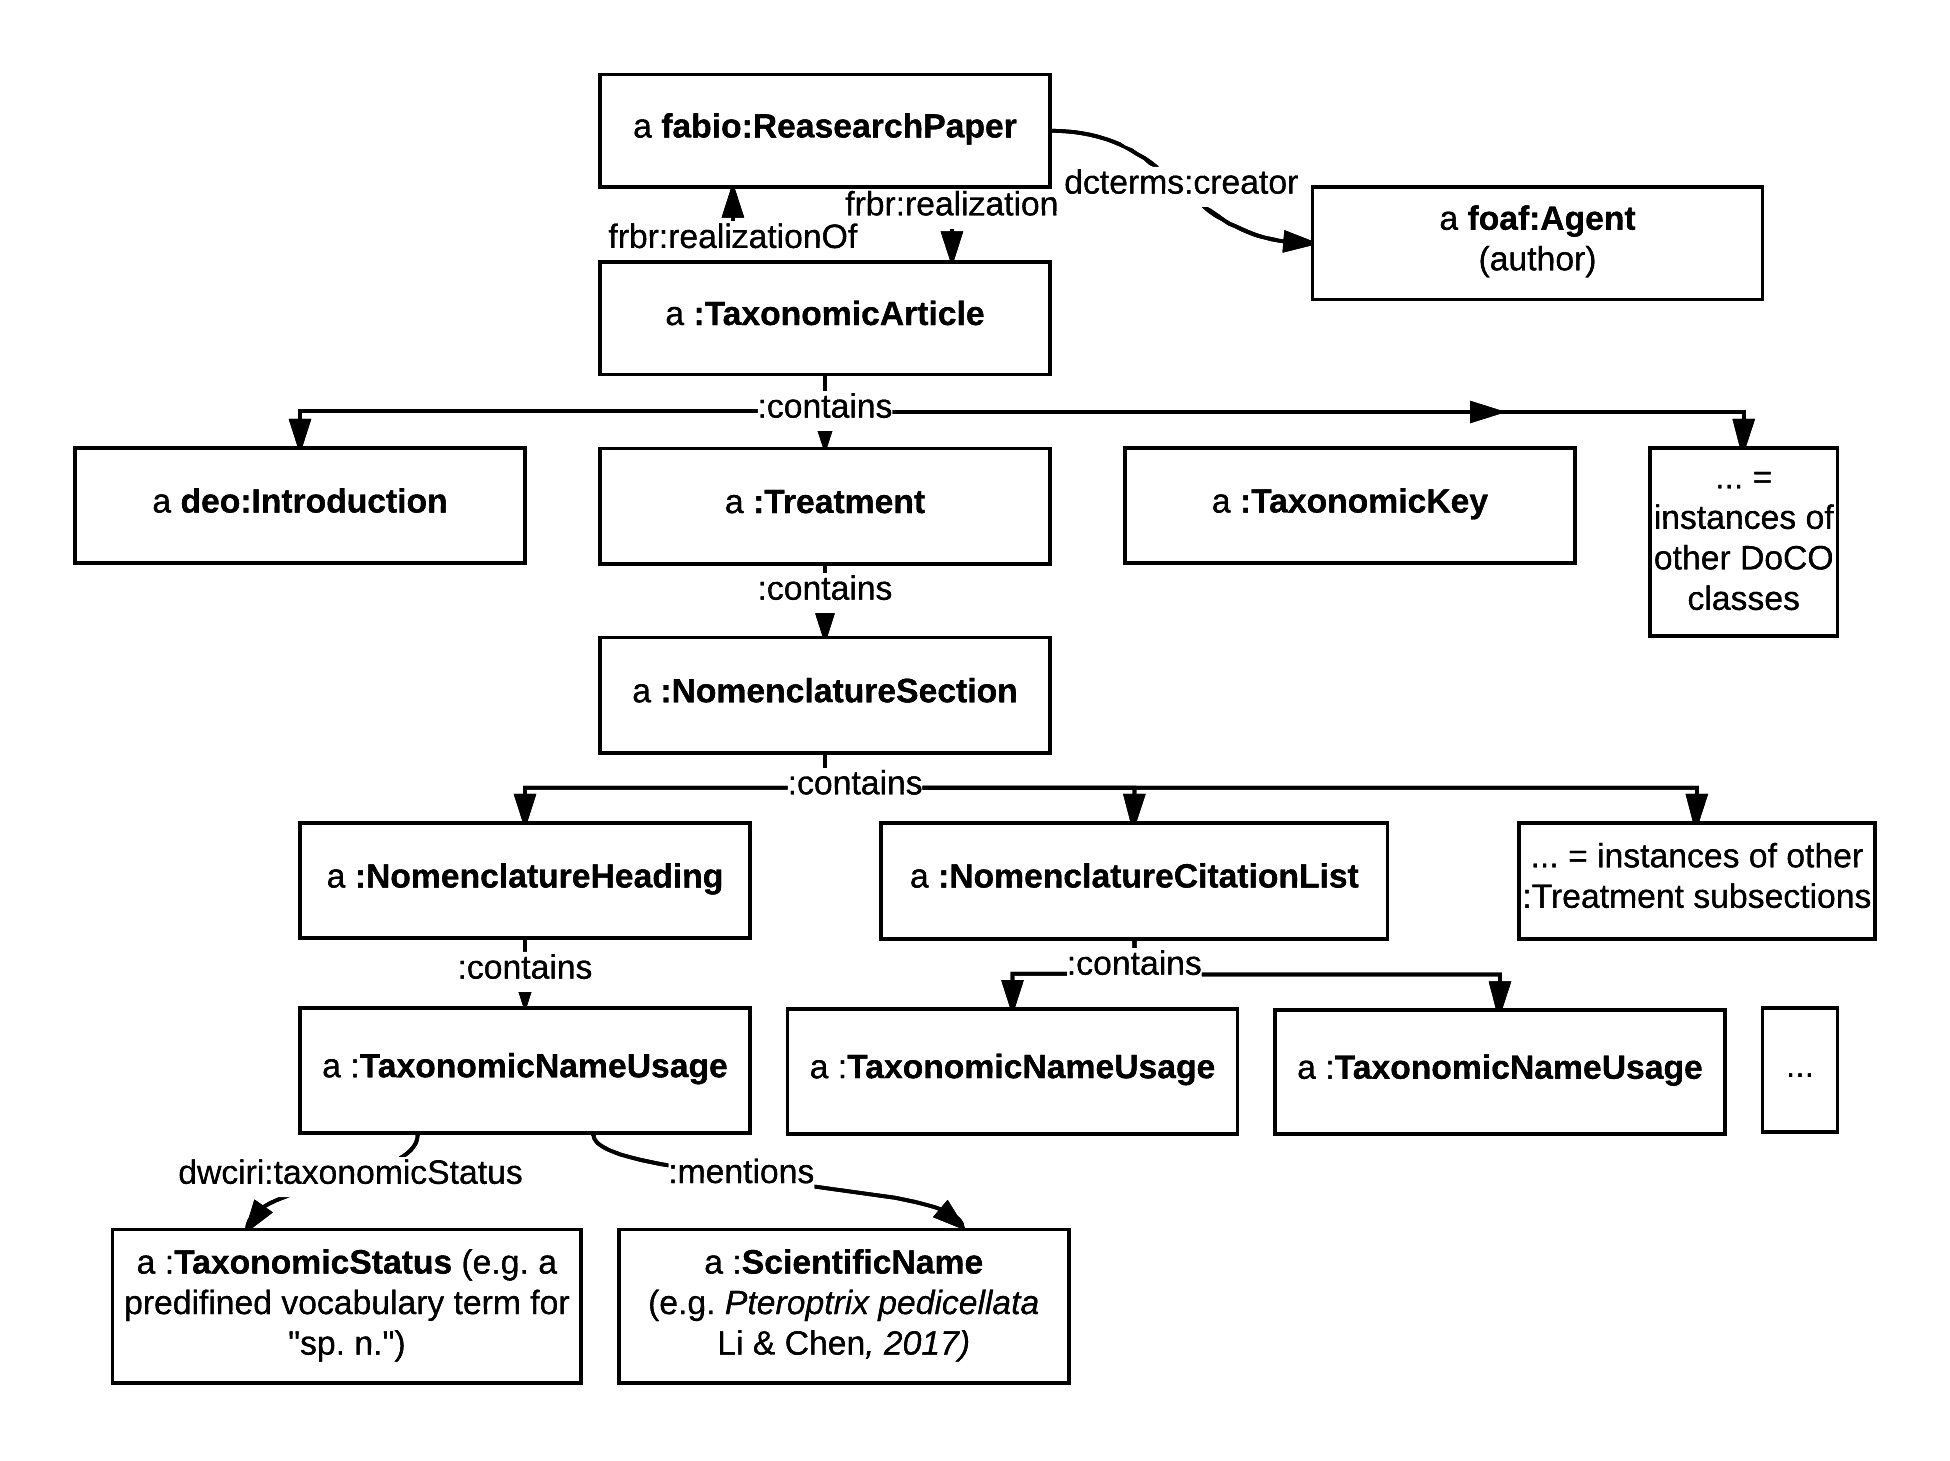
\includegraphics[width=\textwidth]{Figures/taxonomic-article-diagram}
	\decoRule
  \caption[Taxonomic article diagram.]{Графична представяне на взаимоотношенията между ресурсите, които OpenBiodiv въвежда за публикуване на данни за биоразнообразието.}
  \label{taxonomic-article-diagram}
\end{figure}

\subsubsection{Семантика и употреба}

В тази секция ние обсъждаме как класовете и свойствата, които въведохме, са в съответствие с модела на функционалните изисквания за библиографски записи (FRBR), използван от SPAR. Считаме дадена таксономична статия за конкретен израз/запис, FRBR Expression, на абстрактното понятие работа, FRBR Work, представляващо интелектуалното съдържание на статията. Таксономичната дискусия се третира подобно на Въведение, Методи, Резултати и т.н., т.е. също e FRBR Expression и DEO discourse element. Таксономична концепция е съответният абстрактен ресурс от клас FRBR Work на дадена таксономична дискусия. 

\subsection{Семантично моделиране на биологичната номенклатура}

Биологичната номенклатура е система с над 200 годишна традиция датираща до преди времето на информатиката и дори до преди времето на Теорията за еволюцията на Дарвин. Много е трудно да се моделира поради сложността си и само частично е обхваната от онтологиите NOMEN и TNSS (въведени в подраздел ``Previous Work''). С OpenBiodiv-O използвам подход "отдолу-нагоре" за моделиране на използването на таксономични имена в статиите. Където е възможно, ние подравняваме класовете OpenBiodiv-O на NOMEN.

Дефинирахме йерархията на класовете на таксономичните имена, намиращи се на фиг.~\ref{taxonomic-name-class-hierarchy-diagram}. Освен това въведехме taxonomic name usage (\cl{TaxonomicNameUsage}).

\begin{figure}[h!]
  \centering
  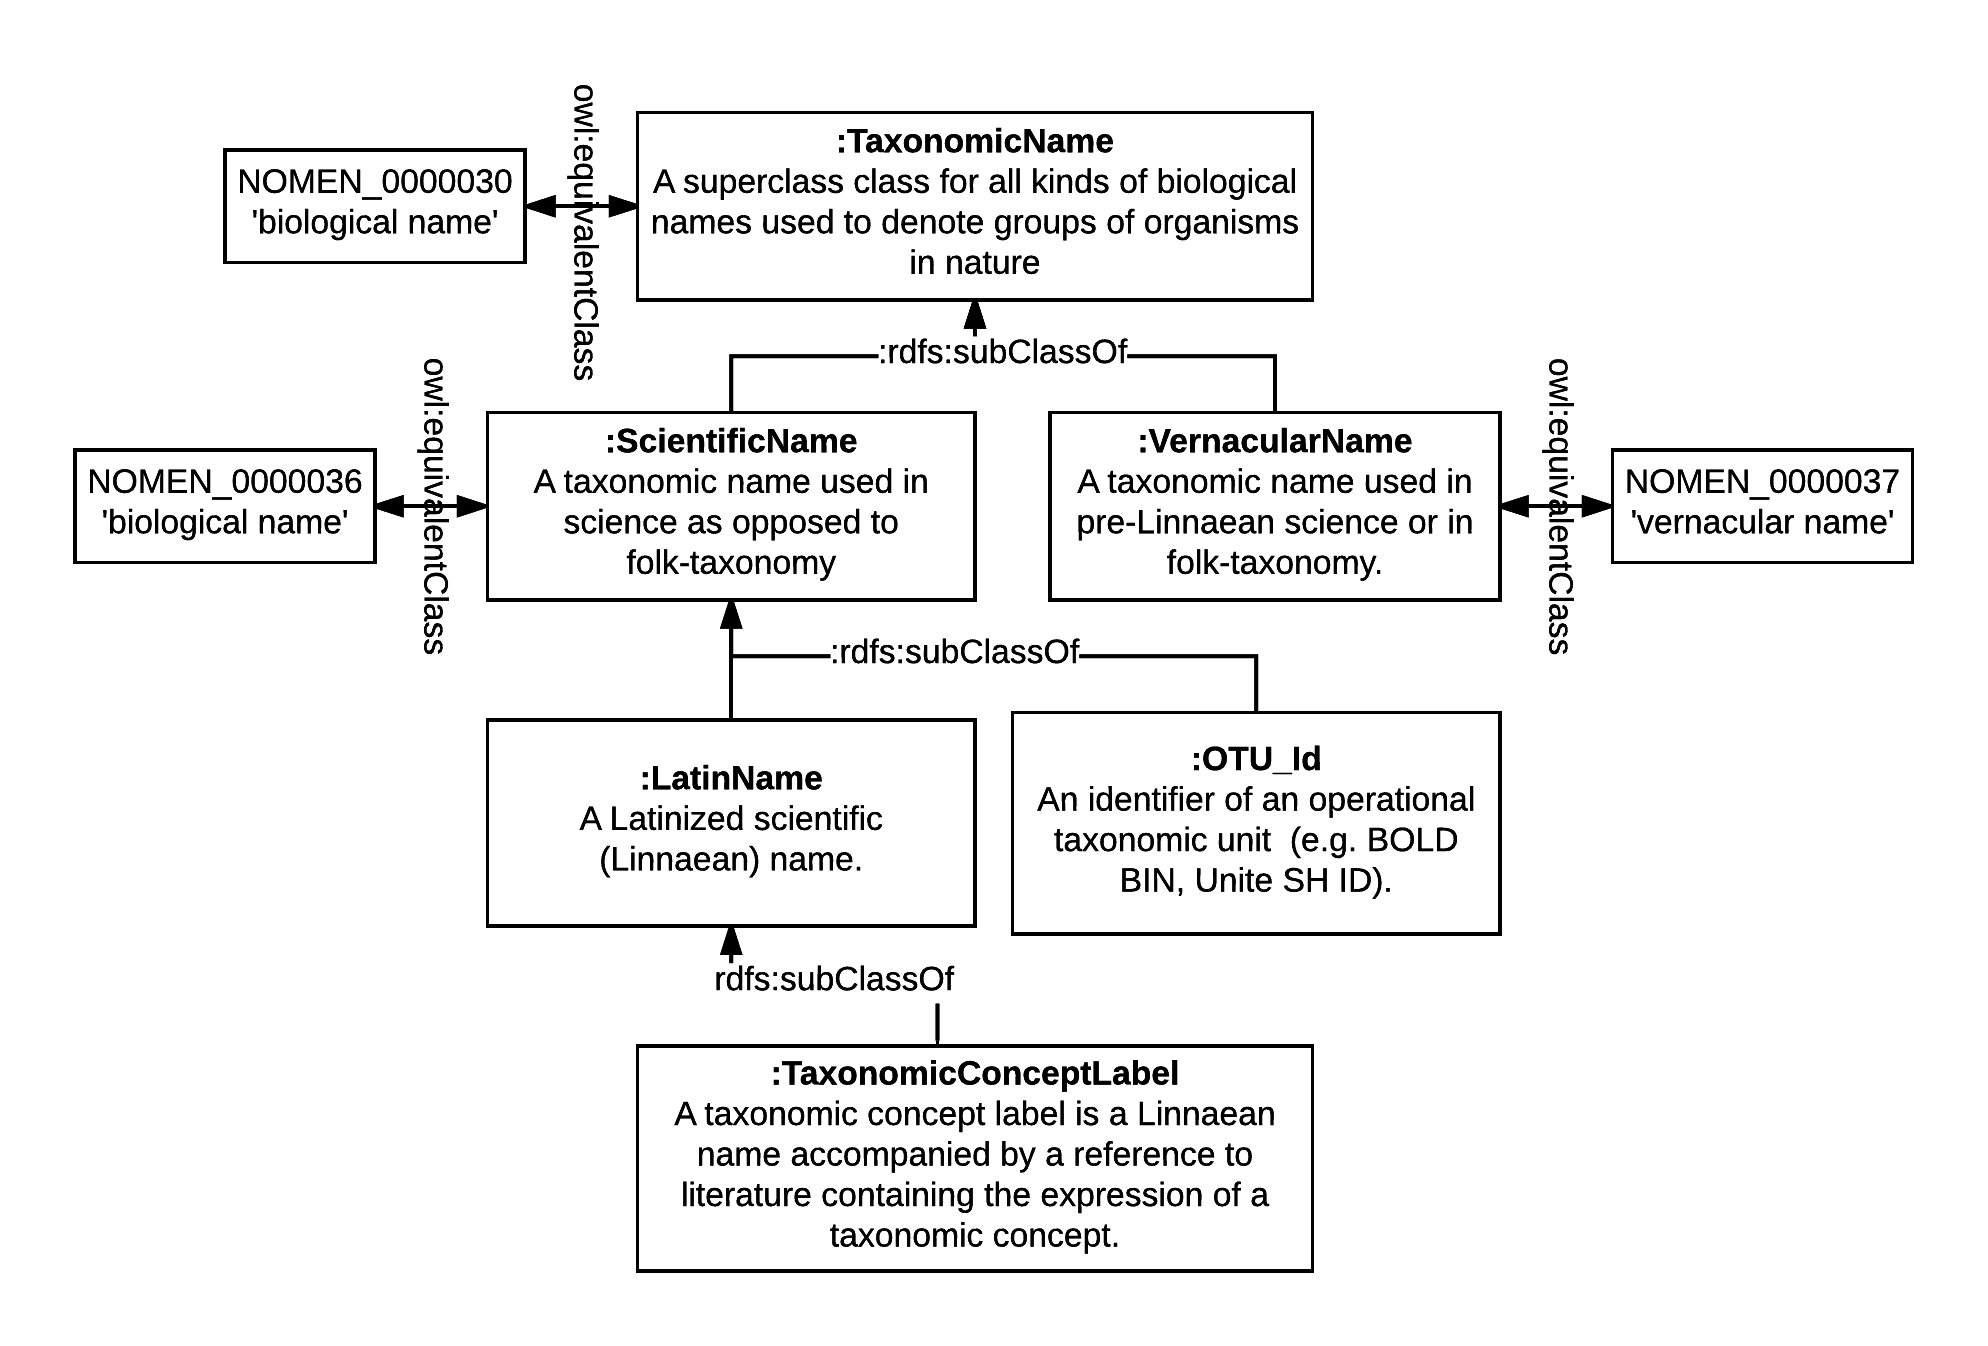
\includegraphics[width=\textwidth]{Figures/taxonomic-name-class-hierarchy-diagram}
  \decoRule
  \caption[Taxonomic name class hierarchy diagram.]{Създадохме тази йерархия, за да приспособим както традиционните таксономични наименования, така и използването на таксономични концептуални етикети и оперативни таксономични единици.}
  \label{taxonomic-name-class-hierarchy-diagram}
\end{figure}

Въвеждаме Taxonomic Concept Label (\cl{TaxonomicConceptLabel}). Етикетът на таксономична концепция (TCL) е линеево име плюс позоваване на публикация, където дискутираният таксон е дефиниран. Връзката се осъществява чрез ключовата дума ``sec.'' (Латинки за (\emph{secundum} \cite{berendsohn_concept_1995}). Напр. \emph{Andropogon virginicus} var. \emph{tenuispatheus} \cite{blomquist_grasses_1948}. Тук \cite{blomquist_grasses_1948} е валидна библиографска справка за публикацията, в която концепцията е дефинирана.

Извадихме съкращения от таксономични термини от около 4000 статии в четири таксономични списания (ZooKeys, Biodiversity Data Journal, PhytoKeys и MycoKeys), за да създадем таксономичен речник на термините, който обхваща осемте най-често срещани случая Таблица~\ref{taxonomic-status-vocabulary}). Латинските съкращения, които са класифицирани в тези класове, могат да бъдат намерени на страницата на OpenBiodiv-O GitHub. (Вижте Методи за повече подробности).

\begin{table}[h!]
\caption{Речник с таксономични термини.}
\begin{tabular}{ccc}
\hline
Vocabulary Instance QName & Example Abbrev & Comment\\ \hline
{\tt :TaxonomicUncertainty} & \emph{incertae sedis} & Taxonomic Uncertainty\\
{\tt :TaxonDiscovery} & \emph{sp. n.} & Taxonomic Discovery \\
{\tt :ReplacementName} & \emph{comb. n.} & Replacement Name \\
{\tt :UnavailableName} & \emph{nomen dubium} &  Unavailable Name \\
{\tt :AvailableName} & \emph{stat. rev.} & Available Name \\
{\tt :TypeSpecimenDesignation} & \emph{lectotype designation} & Type Specimen Designation \\
{\tt :TypeSpeciesDesignation} & \emph{type species} & Type Species Designation\\
{\tt :NewOccurrenceRecord} & \emph{new country record} & New Occurrence Record (for region)\\
\hline
\end{tabular}
\label{taxonomic-status-vocabulary}
\end{table}

Въз основа на нашия анализ на термините за таксономични статуси, идентифицирахме два модела за съответствие между кодирането на латинизираните научни имена (Фиг.~\ref{scientific-name-patterns}). Моделът \emph{заместващо име}, изпълняван чрез свойството \cl{replacementName}, показва, че вместо едно латинизирано име,  трябва да се използва друго. Тя обхваща голямо разнообразие от случаи в кодексите, като например поставянето на един вид таксон в нов род (нова комбинация), поправката на наименование поради номенклатурни причини (ново име), или прилагането на Принципа на приоритет за откриването на синоними ("syn nov.", \cite{international_commission_on_zoological_nomenclature_official_2017}).

\begin{figure}[h!]
 \centering
  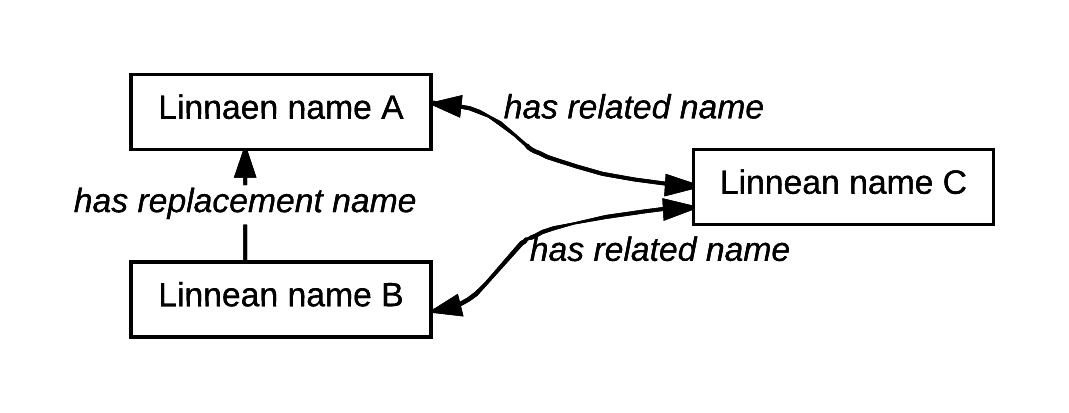
\includegraphics[width=\textwidth]{Figures/scientific-name-patterns}
  \decoRule
  \caption[Scientific name patterns diagram.]{
  Веригите на \emph {заместващи имена} могат да бъдат проследени, за да се намери използваното понастоящем име. \emph{Свързано име} показва, че две имена са свързани по някакъв начин, но не кой е предпочитан.}
  \label{scientific-name-patterns}
\end{figure}

Другият модел е този на \emph{свързани имена} (\cl{relatedName}). Това е по-широк модел, който показва, че две имена са някак си свързани. Например, те могат да бъдат синоними, едното да замества другото, или да сочат към таксономично свързани таксономични понятия. Например, \emph{Harmonia manillana} (\cite{mulsant_monographie_1866}) е свързано с \emph{Caria manillana} \cite {mulsant_monographie_1866} \emph{Harmonia manillana} (според \cite{poorani_harmonia_2016} лектотипус на \emph{Harmonia manillana} (\cite{mulsant_monographie_1866}) sec. \cite{poorani_harmonia_2016} носи името \emph{Caria manillana} \cite{mulsant_monographie_1866}).

\subsubsection{Семантика и употреба}

Както се вижда от фиг.~\ref{taxonomic-name-class-hierarchy-diagram}, таксономичните имена на OpenBiodiv-O са приравнени към NOMEN имена. 


\subsection{Семантично моделиране на таксономичните концепции}

В таксономичните имена на OpenBiodiv-O не са носители на семантична информация за таксоните. Тази задача се изпълнява от нов клас, Taxonomic Concept (\cl{TaxonomicConcept}). Таксономична концепция е теорията, която таксономът формира около таксон посредством научна таксономична публикация. Тя винаги има етикет, състоящ се от таксономичното име и библиографско позоваване на статията, в която името е описано. Въвеждаме и по-общ клас, оперативно таксономично звено (\cl{OperationalTaxonomicUnit}), което може да се използва за всички видове таксономични хипотези, включително такива, които нямат правилен таксономичен етикет . Класовата йерархия е илюстрирана на Фиг.~\ref{taxonomic-concept-diagram}. Свойствата на таксономичните имена са илюстрирани в Фиг.~\ref{name-property-hierarchy}.  Двата начина са изразяване на взаимоотношения между таксономични концепции са дадени във Фиг.~\ref{taxonomic-concept-relationships-diagram}).

\begin{figure}[h!]
\centering
  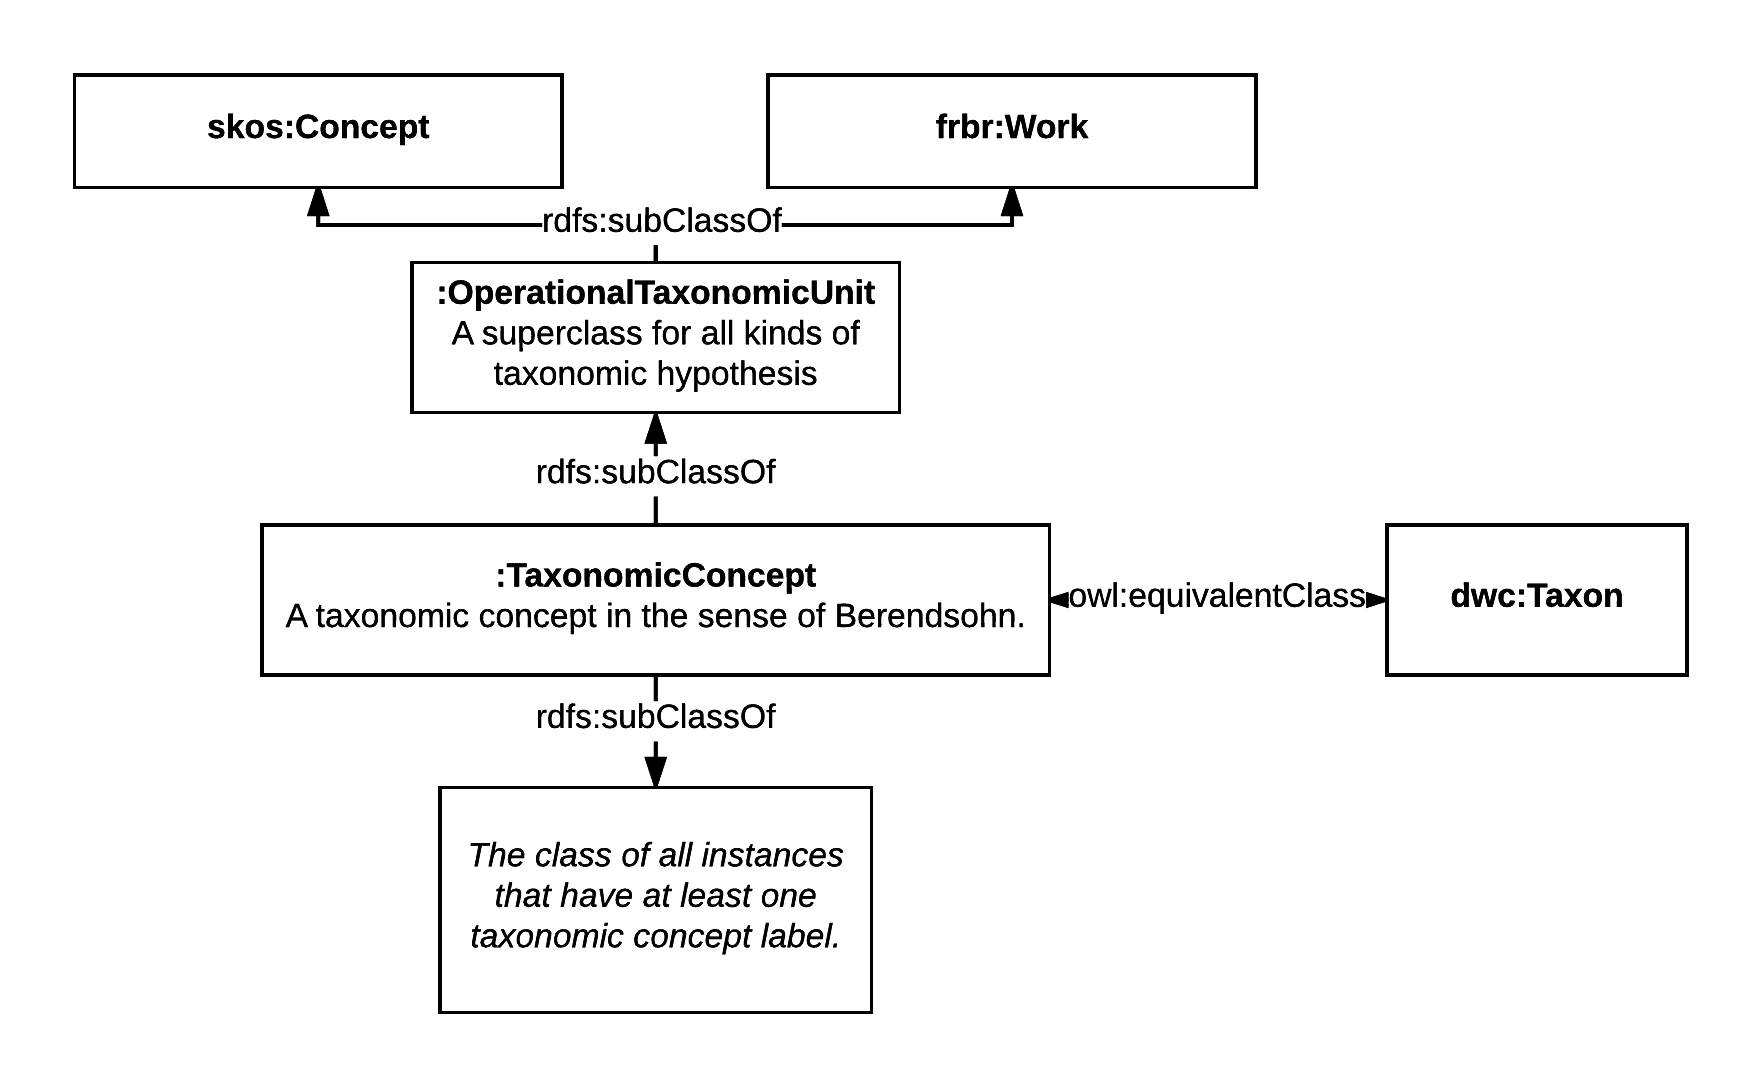
\includegraphics[width=\textwidth]{Figures/taxonomic-concept-diagram}
  \decoRule
  \caption[Taxonomic concept diagram.]{
  Таксономичната концепция е от клас \cl{skos:Concept}, \cl{frbr: Work}, \cl{dwc:Taxon} и има поне един етикет.}
  \label{taxonomic-concept-diagram}
\end{figure}



\begin{figure}[h!]
\centering
  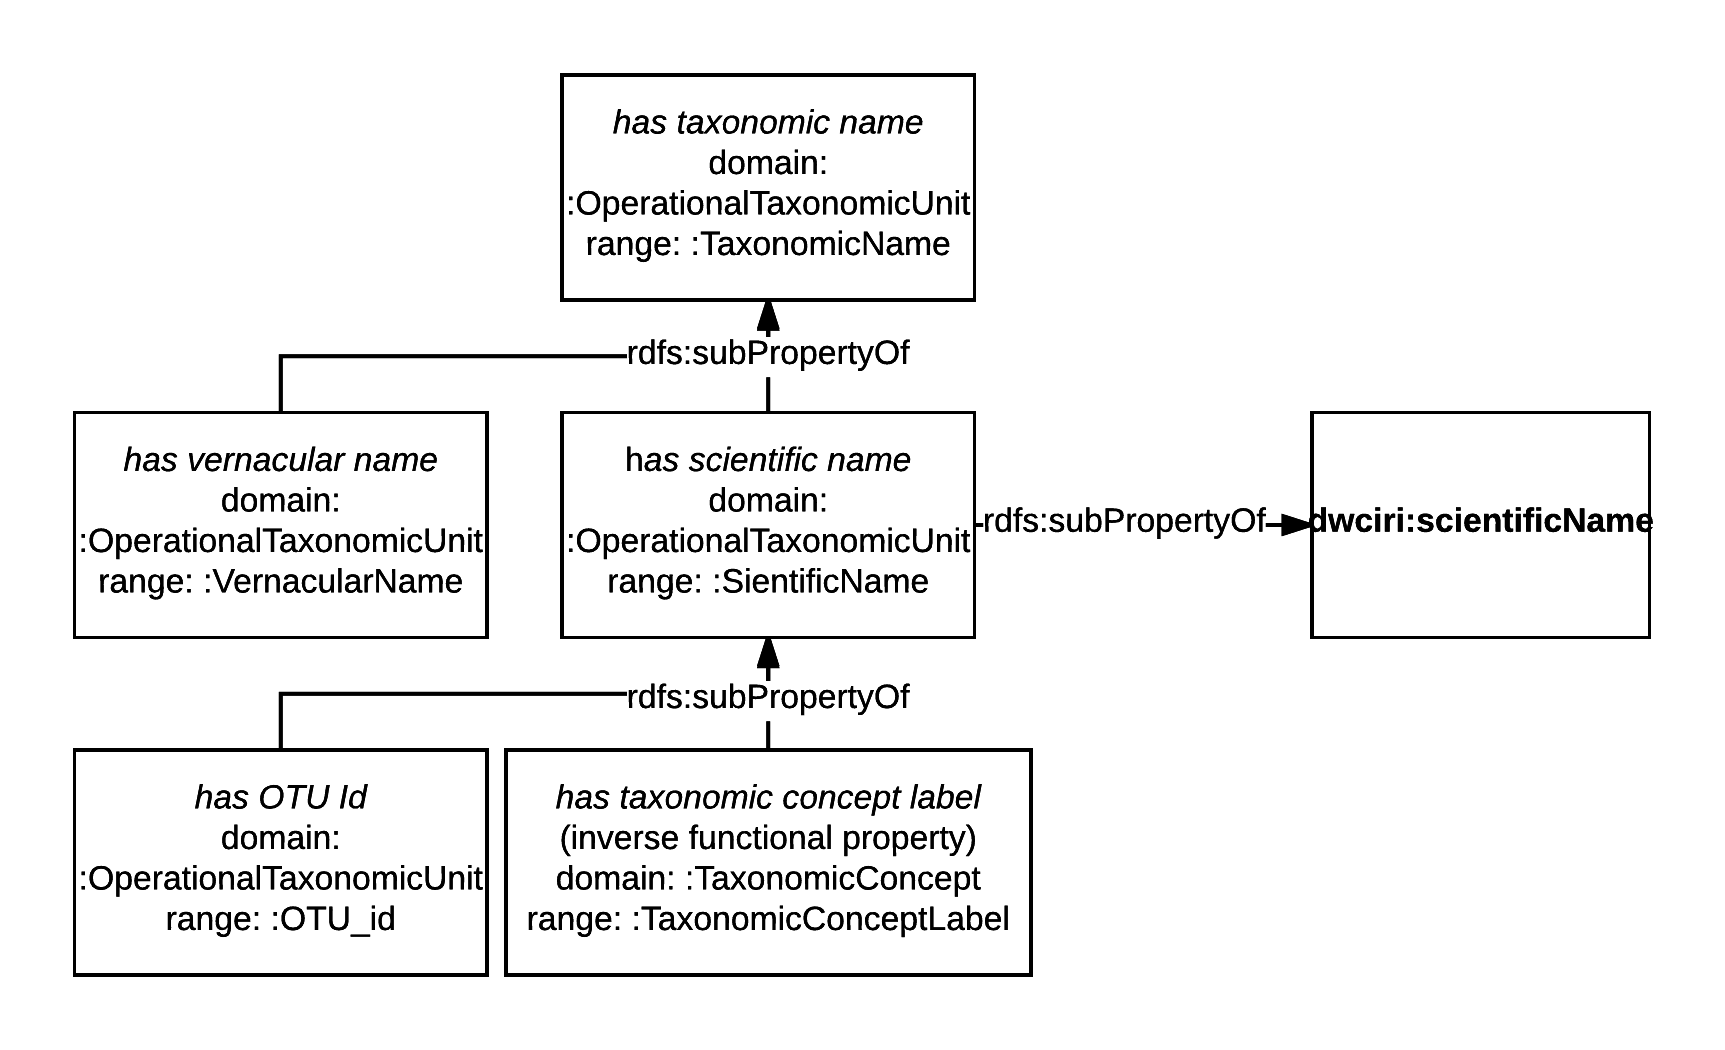
\includegraphics[width=\textwidth]{Figures/name-property-hierarchy}
  \decoRule
  \caption[Taxonomic name property hierarchy diagram.]
  {Йерархията на свойствата съвпада с йерархията на таксономичните имена и е приравнена към DarwinCore.}
  \label{name-property-hierarchy}
\end{figure}



\begin{figure}[h!]
\centering
  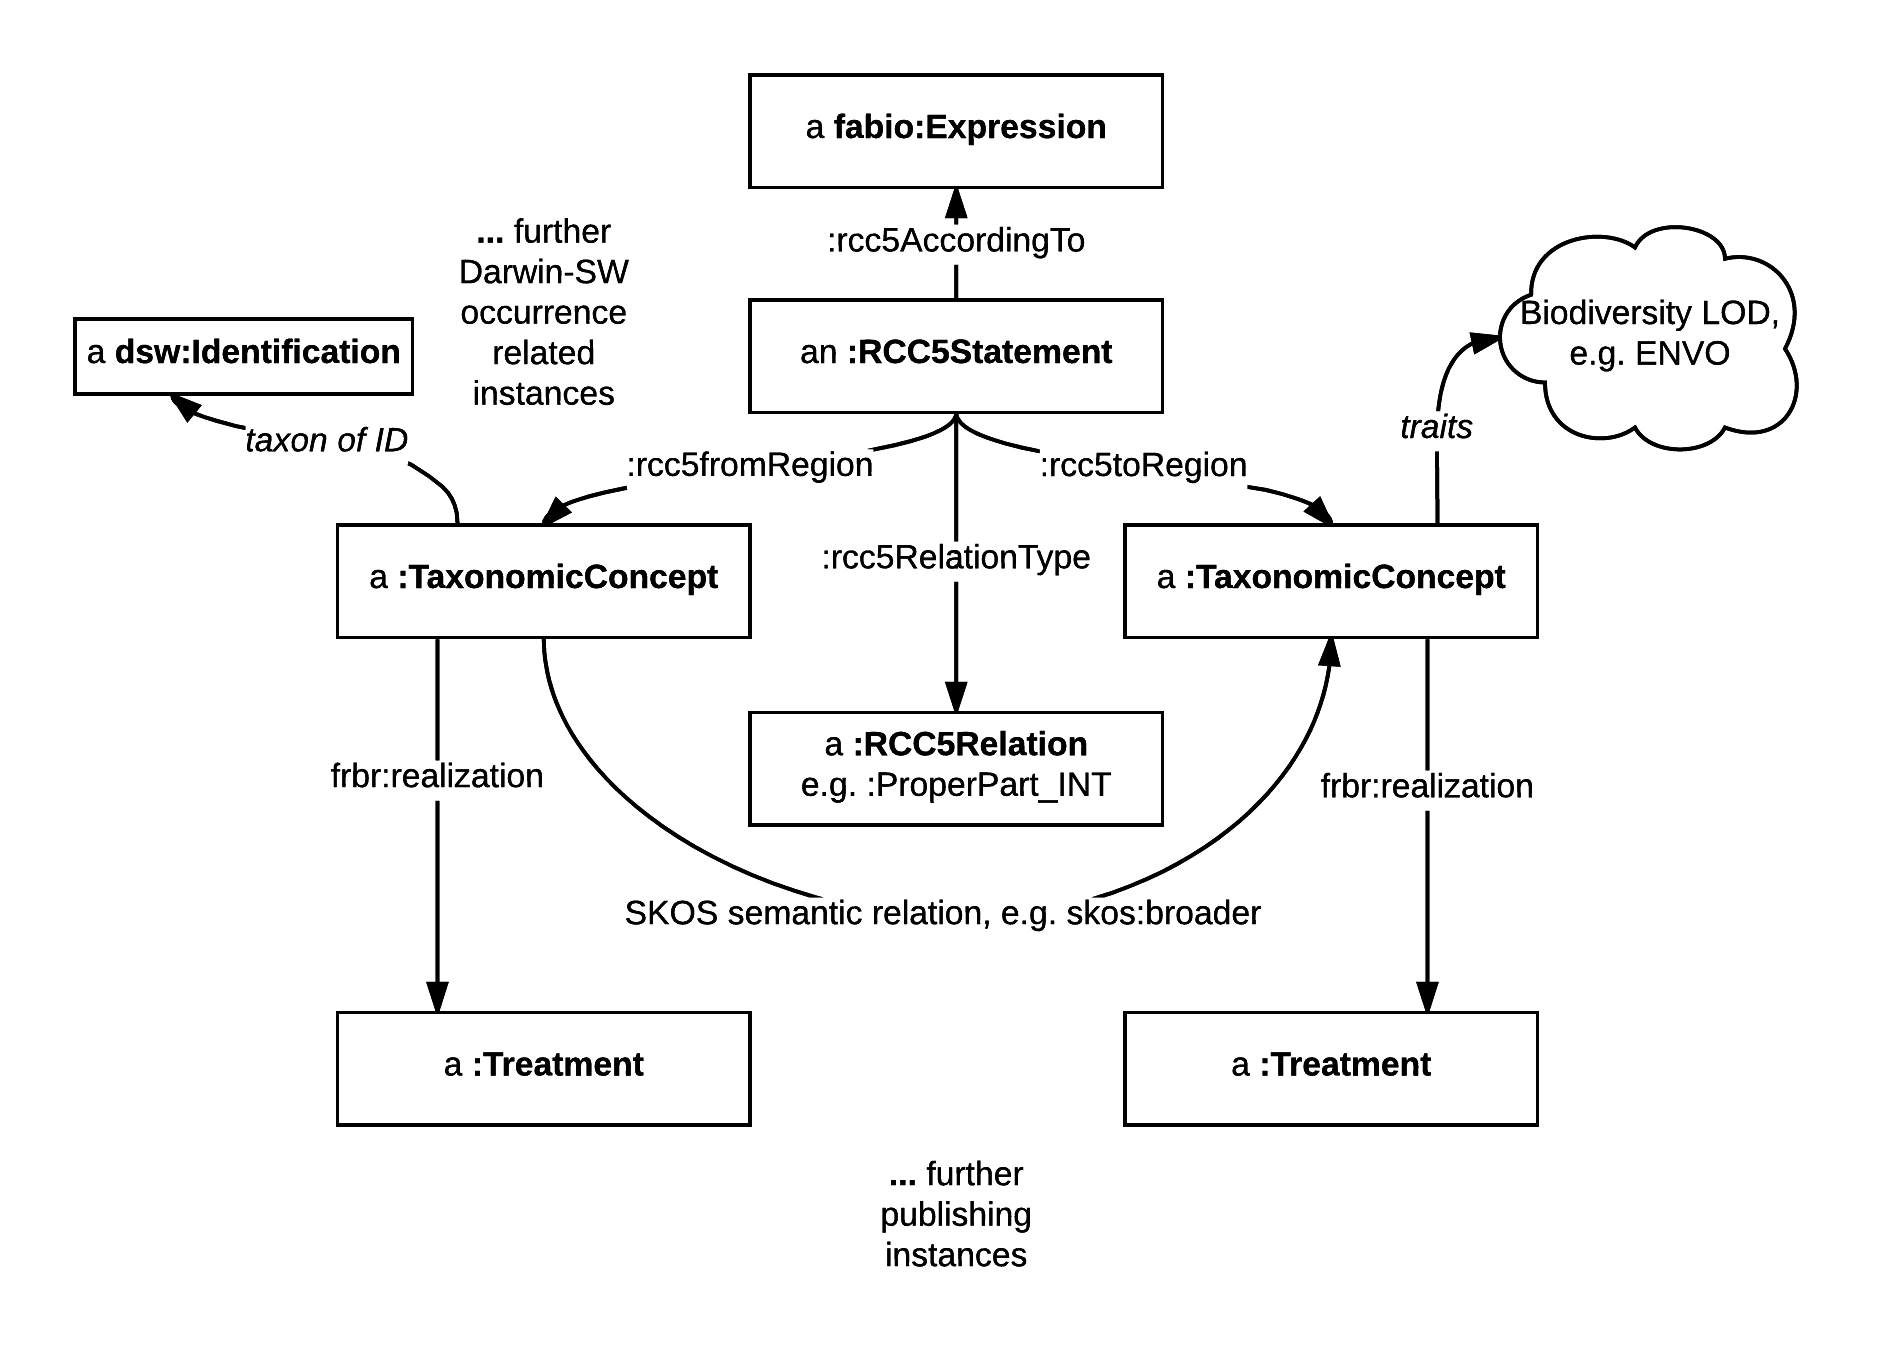
\includegraphics[width=\textwidth]{Figures/taxonomic-concept-relationships-diagram}
  \decoRule
  \caption[Taxonomic concept relationships diagram.]{За да изразите RCC-5 връзка между концепциите, създайте \cl{RCC5Statement} и използвайте съответните свойства, за да свържете две таксономични концепции през него. Освен това, таксономичните понятия са свързани със качества (например екология в ENVO), събития (например Darwin-SW) и са абстрактният клас на Таксономичните дискусии.}
  \label{taxonomic-concept-relationships-diagram}
\end{figure}

Простите отношения не са подходящи за машинен извод. Ето защо \cite{franz_perspectives:_2009}, позовавайки се на \cite{koperski_referenzliste_2000} предложиха да използваме езика RCC-5, за да изразим взаимоотношенията между таксономичните понятия. Тяхни колеги разработиха програмата Euler (\cite{chen_euler/x:_2014}), която използва Answer Set Programming (ASP) за разсъждения и извод по таксономичните взаимоотношения, стъпвайки на RCC-5. Изводната машина за RCC-5 не е част от OpenBiodiv, тъй като тази задача може да бъде изпълнена от Ойлер; въпреки това, ние предоставихме RCC-5 терминилогичен речник. Вж. Фиг.~\ref{example-rcc5-taxonomic-concept-relationships}.

\subsubsection{Семантика и приравняване}

В тази секция таксономичните понятия са приведени в съответствие с DarwinCore (DwC) и е проведена дискусия за това как са представени таксономичните понятия, свързани както с прости отношения (SKOS), така и в подходящ за извод вид (RCC-5). Също така се обсъждат взаимоотношенията между биологичните имена и таксономичните концепции.


\section{Дискусия}

Обсъжда се как OpenBiodiv-O е първият по рода си опит да се моделира онтологично таксономичната публикация. Тя проправя пътя към създаване на граф от знания за биологичното разнообразие.

\section{Заключение}

Главата предоставя концептуализация на таксономичния процес и формализация в OpenBiodiv-O. Въвеждат се класове и свойства в областта на публикуването на биоразнообразие и биологичната систематика и ги привежда в съответствие с важните онтологии, специфични за този домейн.